\documentclass[10pt,letterpaper]{article}
\usepackage[utf8]{inputenc}
\usepackage[spanish]{babel}
\usepackage{listings}
\usepackage{graphicx}
\graphicspath{ {images/} }
\usepackage{cite}
\usepackage{hyperref}
\usepackage{lipsum}
\usepackage{amsmath, amsthm, amssymb}
\usepackage{ragged2e}
\usepackage{fancyhdr}
\usepackage{subfig}
\usepackage{multirow, array}

\begin{document}
	
	%PORTADA
	\pagestyle{empty}
	
	\begin{figure}[h]
		\centering
		
\includegraphics[scale=0.12]{images/escudoUdeA.png}
	\end{figure}
	
	\centering
	
	\textbf{\Large{NOCIONES DE LA MEMORIA DEL COMPUTADOR}}\\
	\vspace{1cm}
	\textbf{\Large{INFORMATICA 2}}\\
	\large
	\vspace{1.4cm}
	\textbf{Juan David Rendon Berrio}\\\vspace{0.1cm}C.C 1037595192 \\\vspace{1cm}      
	
	\textbf{Augusto Salazar}\\
	\vspace{0.2cm}
	\textbf{Jonathan Gómez}\\
	\vspace{0.2cm}
	\Large{Docentes}\\
	\vspace{1cm}
	\vfill
	\large{DEPARTAMENTO DE INGENIERÍA ELECTRÓNICA Y TELECOMUNICACIONES}\\
	\vspace{0.3cm}
	\large{FACULTAD DE INGENIERÍA}\\
	\large{UNIVERSIDAD DE ANTIOQUIA}\\
	\vspace{0.3cm}
	\large{MEDELLIN}\\
	\large{2020-1}\\

\tableofcontents

\newpage
\section{Introducción}

\begin{justify}
	Uno de los grandes temas que tienen que ver con el mundo de la informática, y en lo que todos pensamos ya sea cuando vamos a comprar un computador, o cualquier aparato electrónico; es ¿y cuanta memoria tiene?, pero, en realidad estamos diciendo una palabra sin pensar en su profundidad.\\
	
	\noindent
	La memoria cumple muchas funciones en el mundo de la informática, pero lo primero que se nos viene a la mente para darle significado a esta palabra, es que la memoria es donde uno guarda cosas, cualquier tipo de información, recuerdos, y demás cosas valiosas que uno quiere conservar.\\
	
	\noindent
	En el mundo informático, la memoria cumple varios papeles importantes, en diferentes ámbitos, desde guardar archivos, hasta capacidad de acceso.\\
	
	\noindent
	En este documento se intentará exponer de una manera amigable el significado de la memoria, como funciona, los diferentes tipos que existen, las funciones que desempeña en los diferentes dispositivos electrónicos.
\end{justify}

\newpage
\section{Definición de la memoria del computador} \label{contenido}

\begin{justify}
	Hablando un poco de memoria, es un dispositivo de hardware que retiene datos informáticos de manera permanente o temporal, de acuerdo al tipo, y funcionamiento.\\
	
	\noindent
	Las memorias de computadora, o hablando un poco mas general, de cualquier dispositivo electrónico, proporcionan una de las principales funciones de la computación moderna; la retención o el almacenamiento de información. Es uno de los componentes fundamentales de todas las computadoras, que acoplada a una unidad central de procesamiento (CPU), por su sigla en inglés, “Central processing unit”, implementa lo fundamental del modelo de computadora de Arquitectura de von Neumann, usado desde los años 1940.\cite{primera} \\ 
	
	\noindent
	En cuanto al hardware, existen en el mercado muchos tipos de memoria creados y desarrollados para suplir varias necesidades que se fueron presentando en toda la arquitectura computacional.
	
\end{justify}
 
\newpage
\section{Tipos de Memoria} \label{contenido}


\begin{justify}
	En un computador hay varios tipos de memoria, ordenados en jerarquías de velocidad y capacidad.\\
	
	\begin{itemize}
		\item Memoria Cache L1, L2 y L3
		\item Memoria RAM 
		\item Memoria Virtual 
		\item Disco Duro 		
	\end{itemize}
	Cuanto más bajamos en la lista desde la memoria Cache hacia el disco duro, decrece la velocidad de los distintos tipos de memoria y aumenta su capacidad.\\
	
	\begin{center}
	\textbf{Memoria cache}
	\end{center}

	\begin{figure}[h]
		\centering
		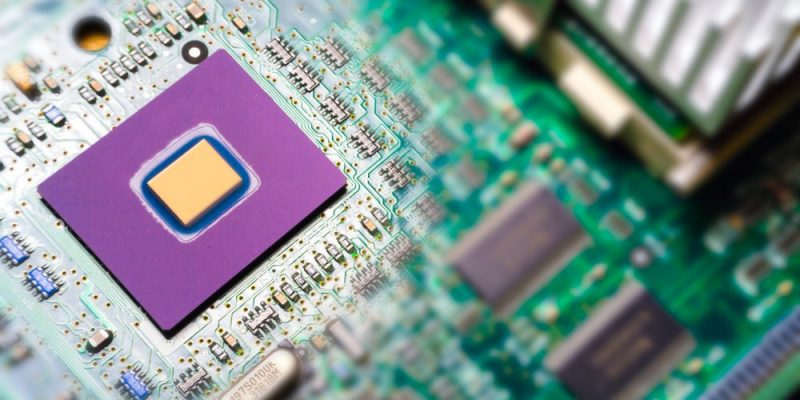
\includegraphics[scale=0.3]{images/cache.jpg}
	\end{figure}
	
	\noindent
	En \underline{informática}, se conoce como \textbf{memoria caché} o memoria de acceso rápido a uno de los recursos con los que cuenta una CPU (Central Processing Unit, o sea, Unidad Central de Procesamiento) para almacenar temporalmente los datos recientemente procesados en un búfer especial, es decir, en una memoria auxiliar.\cite{segunda} \\ 
	
	\noindent
	La memoria caché opera de modo similar a la Memoria Principal del CPU, pero con mayor velocidad a pesar de ser de mucho menor tamaño. Su eficacia \textbf{provee al microprocesador de tiempo extra para acceder a los datos más frecuentemente utilizados}, sin tener que rastrearlos a su lugar de origen cada vez que sean necesarios.\\
	
	\noindent
	Así, esta memoria alterna \textbf{se sitúa entre el CPU y la Memoria RAM} (Random Access Memory, o sea, Memoria de Acceso Aleatorio), y provee de un empuje adicional en tiempo y ahorro de recursos al sistema. De allí su nombre, que en inglés significa “escondite”.\\
	
	\noindent
	Existen varios tipos de memoria caché, como los siguientes:\\
	
	\begin{itemize}	
	\item \textbf{Caché de disco:} Es una porción de memoria RAM asociada a un disco particular, en donde se almacenan los datos de reciente acceso para agilizar su carga.\\
	\item \textbf{Caché de pista:} Similar a la RAM, este tipo de memoria caché sólida empleada por supercomputadores es potente, pero costosa.\\
	\item \textbf{Caché de Web:} Se ocupa de almacenar los datos de las páginas Web recientemente visitadas, para agilizar su carga sucesiva y ahorrar ancho de banda. Este tipo de caché a su vez puede funcionar para un solo usuario (privada), varios usuarios a la vez (compartida) o en conjunto para toda la red administrada por un servidor (en pasarela).
	\end{itemize}

	\noindent
	La Memoria Cache es muy rápida y también muy costosa ya que utiliza más componentes que la memoria común y también es físicamente más grande. Esta es categorizada en niveles que describen que tan cercana está al microprocesador.\cite{tercera} \\ 
	
	\noindent
	\textbf{Memoria Cache Nivel 1 (L1):}
	Esta memoria cache es extremadamente rápida pero relativamente pequeña y hoy día se encuentra integrada en el CPU (años atrás podía o no estar integrada en el CPU). Todas las instrucciones se buscan primero aquí, si no están presentes entonces se procede al siguiente nivel.\\
	
	\noindent
	\textbf{Memoria Cache Nivel 2 (L2):}
	Esta memoria cache es considerablemente más grande que L1 y también está dentro del CPU (años atrás no lo estaba). Si las instrucciones no fueron encontradas en el Nivel L1 entonces se buscan en este Nivel L2, este tipo de memoria no es tan rápida como la usada en L1 por tanto es de esperar un poco de latencia (demora).\\
	
	\noindent
	\textbf{Memoria Cache Nivel 3 (L3):}
	Este es un nivel de memoria especializada que ayuda a mejorar el rendimiento de los Niveles de Cache L1 y L2. Es mucho más lenta que la memoria L1 o L2, pero mucho más rápida que la memoria RAM del Sistema. En el caso de los Procesadores con muchos Cores, cada uno de ellos tiene su propio Cache L1 y Cache L2, pero, todos comparten el mismo Cache L3. Cuando una instrucción es buscada en L3 se eleva a un cache de un nivel más alto.\\
	
	\newpage
	
	\begin{center}
		\textbf{¿Cómo funciona la memoria caché?}
	\end{center}

	\begin{figure}[h]
	\centering
	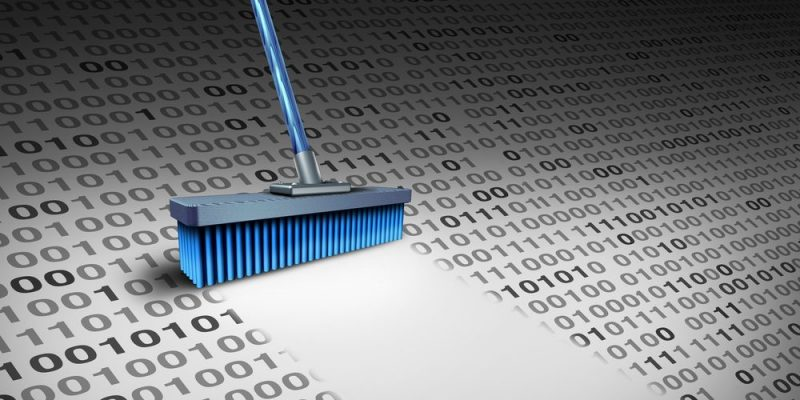
\includegraphics[scale=0.35]{images/funcionamiento.jpg}
	\end{figure}

	El funcionamiento de esta memoria alterna es simple: cuando accedemos a un dato cualquiera en nuestro sistema computarizado, se crea de inmediato una copia de los datos más relevantes del mismo en la memoria caché, de modo que los accesos siguientes a dicha \underline{información} la tengan a mano y no deban rastrearla hacia su lugar de origen.\\

	\noindent
	Así, accediendo a la copia y no al original, se ahorra tiempo de procesamiento y por ende velocidad, ya que el microprocesador no debe acudir todo el tiempo a la memoria principal. Se trata, digámoslo así, de \textbf{una copia de trabajo constantemente actualizada de los datos} de más frecuente utilización.\\

	\newpage
\begin{center}
	\textbf{¿Qué es y por qué es importante la memoria RAM?}
	\end{center}
	
	\begin{figure}[h]
		\centering
		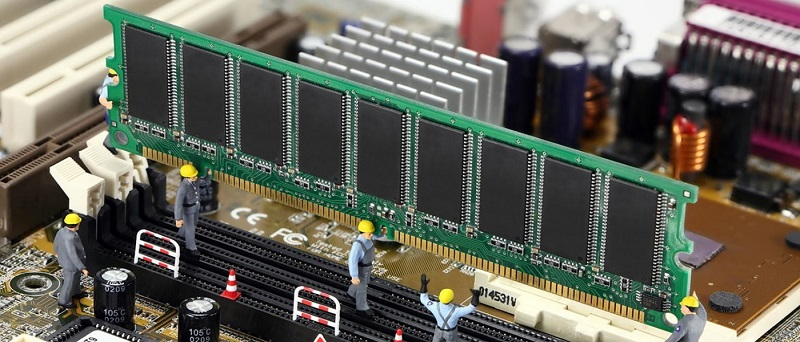
\includegraphics[scale=0.5]{images/ram1.jpg}
	\end{figure}

	\noindent
	Su importancia está fuera de toda duda, ya que aunque ejerce una función distinta a la del procesador, no solo resulta básico para poder utilizar un PC (o cualquier dispositivo electrónico), sino que además juega un papel fundamental en el rendimiento del sistema.\cite{cuarta} \\
	
	\noindent	
	RAM son las siglas de «Random Access Memory» o «Memoria de Acceso Aleatorio». Su formato más extendido es el de \textbf{un PCB a modo de pastilla rectangular} sobre el que se asientan diferentes chips que contienen cantidades determinadas de memoria RAM.\\

	\noindent
	La memoria RAM siempre se ha medido partiendo de un pilar básico: su capacidad. Los \textbf{kilobytes} fueron el nivel más utilizado entre finales de los setenta y principios de los ochenta. Posteriormente dejaron paso a los \textbf{megabytes} y finalmente llegamos a los \textbf{gigabytes}, que es la medida que utilizamos actualmente, aunque ya empezamos a hablar de terabytes en el sector profesional.\\
	\noindent
	
	Como el procesador la memoria RAM se inserta en la placa base y se comunica con diversos elementos del sistema. Su función principal es \textbf{almacenar datos e instrucciones} para que puedan ser accedidos por otros componentes básicos, de manera que evita que tengan que volver a pasar por el procesador o incluso por la tarjeta gráfica.\\
	
	\noindent
	Podemos entender mejor su funcionamiento con un ejemplo sencillo. Cuando encendemos el PC y arrancamos un juego éste carga una serie de datos básicos que necesita en la memoria RAM, y se mantienen en ella \textbf{de forma permanente o hasta que necesita sustituirlos} por otros datos (por ejemplo al cambiar de misión o de mundo e iniciar un nuevo proceso de carga). De esta forma se eliminan las cargas constantes y se consigue un rendimiento y una fluidez óptima.\\
	
	\noindent
	La capacidad de la memoria RAM es fundamental, de hecho es lo primero que debemos priorizar a la hora de comprar, ya que si no tenemos la capacidad mínima que exigen determinadas aplicaciones y juegos no disfrutaremos de una buena experiencia, y en el peor de los casos \textbf{ni siquiera podremos iniciarlas}.\\ 
	
	\noindent
	Los sistemas operativos modernos cuentan con sistemas de memoria virtual que permite utilizar una parte del sistema de almacenamiento (HDD o SSD) para cubrir las carencias de memoria RAM, pero no obrará milagros si no llegamos a un mínimo.\\
	
	\noindent
	Es importante tener en cuenta además que la memoria RAM es un tipo de memoria volátil, lo que significa que a diferencia de los \textbf{HDDs} o los \textbf{SSDs} pierde la información almacenada una vez que se apaga.
	
	
	\begin{flushleft}
		\textbf{Memoria RAM: capacidad?}	
		\end{flushleft}
		
		\noindent
		Hemos dicho que la capacidad (o la cantidad) de memoria RAM es lo primero que debemos tener en cuenta, pero debemos recordar que hay \textbf{diferentes niveles} que podemos considerar como óptimos en función de lo que vayamos a hacer con el PC.\\
		
		\noindent
		Hoy por hoy lo más normal es encontrar módulos de memoria con configuraciones mínimas de \textbf{1 GB} y kits con configuraciones mínimas de \textbf{4 GB} (dos módulos de 2 GB cada uno). A continuación os dejamos un listado con las cantidades recomendadas para disfrutar de una buena experiencia de uso en diferentes entornos y con distintas aplicaciones.\\
				
		\begin{itemize}
			\item Trabajo básico en Word, navegación por Internet y contenidos multimedia sencillos: tendremos suficiente con \textbf{2 GB de RAM}.
			\item Trabajo con documentos complejos, navegación web con varias pestañas, contenidos multimedia y multitarea moderada: debemos contar al menos con \textbf{4 GB de RAM}.
			\item Trabajo con cualquier tipo de documentos, navegación web con decenas de pestañas, juegos, contenidos multimedia y multitarea alta: es necesario contar con \textbf{8 GB de RAM}.
			\item Trabajo con aplicaciones intensivas (edición de fotos y vídeo), juegos muy exigentes, multitarea y contenidos multimedia: es recomendable contar con \textbf{16 GB de RAM}.
			
		\end{itemize}
	
	\begin{center}
		\textbf{¿Qué es la memoria ROM?}
	\end{center}
	En informática, cuando hablamos de memoria ROM (acrónimo de Read–Only Memory, es decir, Memoria de Sólo Lectura), nos referimos a \textbf{un tipo de almacenamiento empleado en computadores y otros dispositivos electrónicos}, que se caracteriza por ser únicamente de acceso para lectura y nunca para escritura, es decir, que se la puede recuperar pero no modificar o intervenir. \\
	
	\noindent
	La memoria ROM es de acceso secuencial y su presencia es independiente de la presencia de una fuente de energía. Como se ha dicho, \textbf{su contenido no puede modificarse}, o al menos no de manera simple y cotidiana, y suele contener información introducida en el sistema por el fabricante, de tipo básico, operativo o primario. \\
	
	\noindent
	Este tipo de memoria opera, además, de manera \textbf{mucho más lenta que su contrapartida, la RAM} (acrónimo de Random Access Memory, es decir, Memoria de Acceso Aleatorio), por lo que su contenido suele volcarse en esta última para ejecutarse más velozmente. \\
	
	\noindent
	Existen, no obstante, versiones de memoria ROM (conocidas como EPROM y Flash EEPROM) que \textbf{pueden ser programadas y reprogramadas varias veces}, a pesar de que su funcionamiento se rige por las mismas reglas del tradicional. Sin embargo, como su proceso de reprogramación es poco frecuente y relativamente lento, se las continúa llamando del mismo modo.\\
	
	\newpage
	\begin{center}
		\textbf{¿Para qué sirve la memoria ROM?}
	\end{center}
	
	\noindent
	La memoria ROM tiene dos usos principales, que son:\\
	
	\begin{itemize}
		\item \textbf{Almacenamiento de software:} Comúnmente, los ordenadores en la década de 1980 traían todo su sistema operativo almacenado en ROM, para que los usuarios no pudieran alterarlo por error e interrumpir el funcionamiento de la máquina. Aún hoy en día se la utiliza para instalar el software de arranque o de funcionamiento más básico (el BIOS, SETUP y POST, por ejemplo).
		\item \textbf{Almacenamiento de datos:} Dado que los usuarios no suelen tener acceso al ROM de un sistema, se lo emplea para almacenar los datos que no requerirán de modificación alguna en la vida del producto, como tablas de consulta, operadores matemáticos o lógicos y otra información de índole técnica.
	\end{itemize}
	
	\begin{center}
		\textbf{Tipos de Memoria ROM}
	\end{center}
	
	\noindent
	Consideremos tres tipos distintos de memoria ROM:\\
	
	\begin{itemize}
		\item \textbf{PROM:} Acrónimo de Programmable Read–Only Memory (Memoria de Sólo Lectura Programable), es de tipo digital y puede ser programada una única vez, ya que cada unidad de memoria depende de un fusible que se quema al hacerlo.
		
		\item \textbf{EPROM:} Acrónimo de Erasable Programmable Read–Only Memory (Memoria de Sólo Lectura Borrable y Programable) es una forma de memoria PROM que puede borrarse al exponerse a luz ultravioleta o altos niveles de voltaje, borrando la información contenida y permitiendo su remplazo.
		
		\item \textbf{EEPROM:} Acrónimo de Electrically Erasable Programmable Read-Only Memory (Memoria de Sólo Lectura Borrable y Programable Eléctricamente) es una variante del EPROM que no requiere rayos ultravioleta y puede reprogramarse en el propio circuito, pudiendo acceder a los bits de información de manera individual y no en conjunto.
	\end{itemize}

	\newpage
	\begin{center}
		\textbf{El Disco Duro o unidad de Almacenamiento no volátil}	
	\end{center}
	
	\noindent
	Los discos duros, también conocidos como HDD, son un componente informático que sirve para almacenar de forma permanente tus datos. Esto quiere decir, que los datos no se borran cuando se apaga la unidad como pasa en los almacenados por la memoria RAM. La primera empresa en comercializarlos fue IBM en 1956.\cite{quinta} \\
	
	\noindent
	Están compuestos de piezas mecánicas, de ahí que a veces se le llame discos duros mecánicos, y \textbf{utilizan el magnetismo para grabar tus datos y archivos.} Se compone de uno o varios discos rígidos unidos por un mismo eje y que giran a gran velocidad dentro de una caja metálica. En cada plato y en cada una de sus caras, un cabezal de lectura/escritura lee o graba tus datos sobre los discos. \\
	
	\noindent
	Cuanto más finos sean los discos mejor será la grabación, y cuanto \textbf{más rápido giran a mayor velocidad se transmiten los datos}, tanto a la hora de leerlos como al escribirlos. Por lo general, la velocidad de los discos duros suele ser de 5400 o 7200 RPM (revoluciones por minuto), aunque en algunos discos basados en servidores pueden llegar a hasta 15.000 RPM. \\
	
	\noindent
	Las unidades de estado sólido o SSD (Solid State Drive) son una alternativa a los discos duros. La gran diferencia es que mientras los discos duros utilizan componentes mecánicos que se mueven, \textbf{las SSD almacenan los archivos en microchips con memorias flash interconectadas entre sí.} Por lo tanto, casi podríamos considerarlos como una evolución de las memorias USB. \\
	
	\noindent
	Los SSD suelen utilizar memorias flash basadas en NAND, que como también son no-volátiles mantienen la información almacenada cuando el disco se desconecta. No tienen cabezales físicos para grabar los datos, en su lugar \textbf{incluyen un procesador integrado} para realizar operaciones relacionadas con la lectura y escritura de datos. \\
	
	\noindent
	Estos procesadores, llamados controladores, son los que toman las "decisiones" sobre cómo almacenar, recuperar, almacenar en caché y limpiar los datos del disco, y \textbf{su eficiencia es uno de los factores que determinan la velocidad total de la unidad}. Además, al no depender del giro de un componente físico, también se logra una unidad más silenciosa que los discos mecánicos.\\
	
	\begin{flushleft}
		\textbf{SSD NVMe}
	\end{flushleft}
	
	\begin{figure}[h]
		\centering
		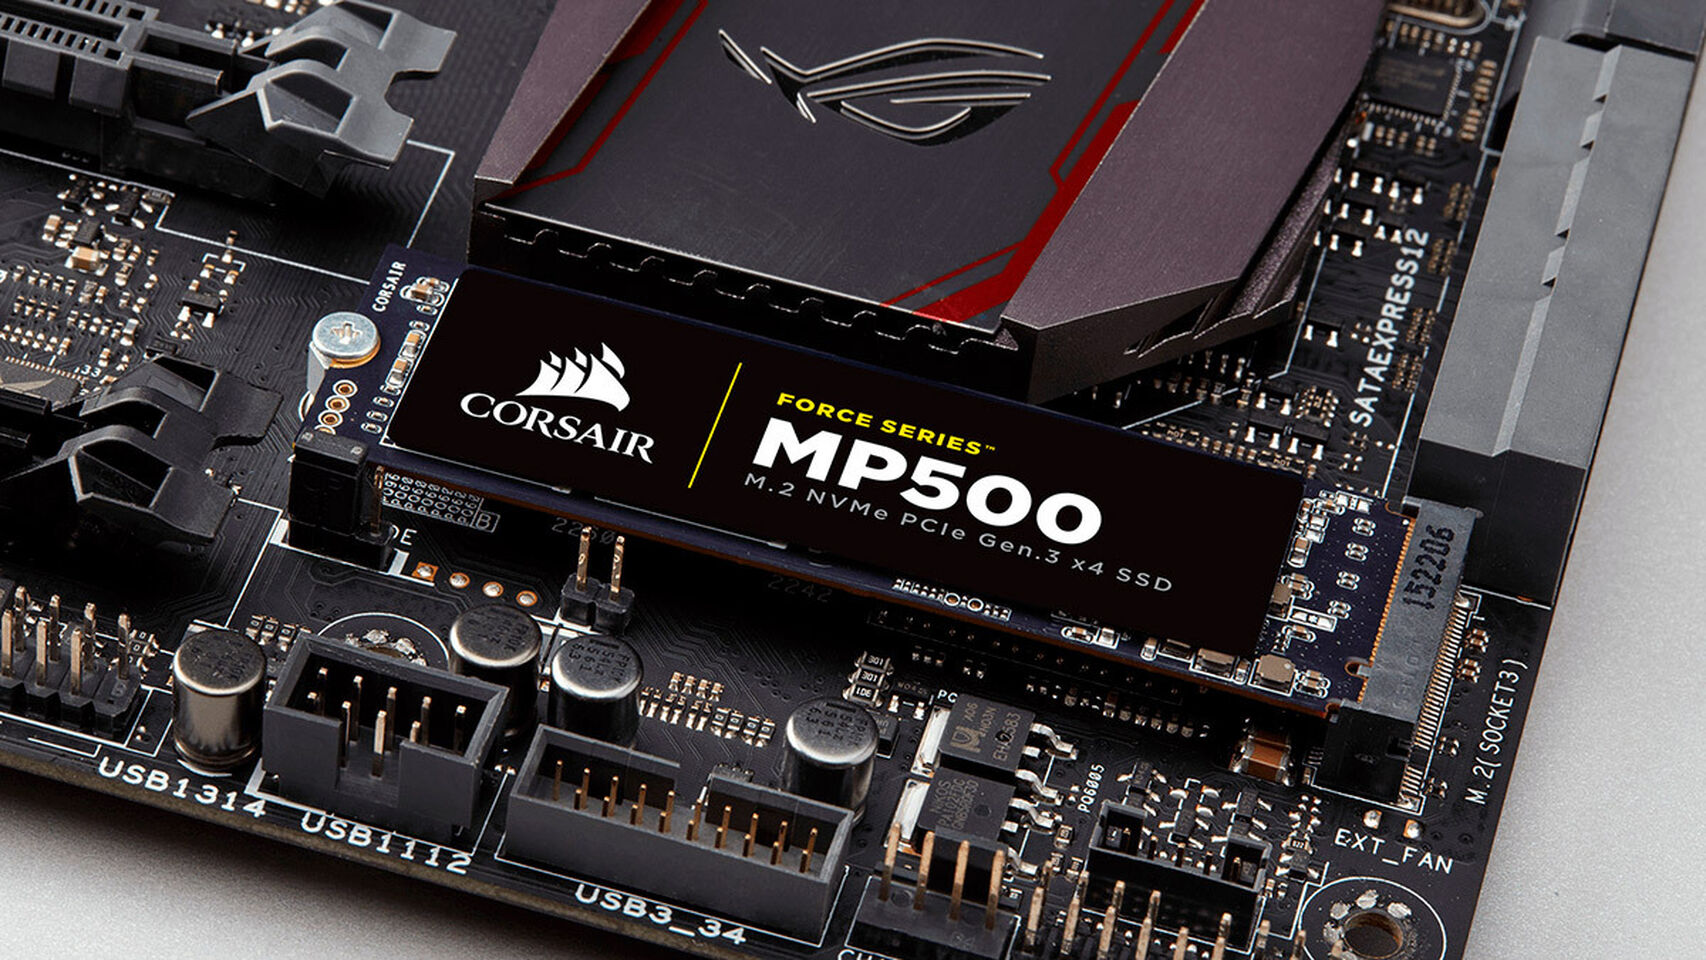
\includegraphics[scale=0.18]{images/ssd.jpg}
	\end{figure}
	
	\noindent
	NVMe (memoria no volátil express) es un nuevo protocolo de transporte y acceso al almacenamiento para unidades flash y de estado sólido (SSD) de nueva generación que ofrece el rendimiento más alto y los tiempos de respuesta más breves para todos los tipos de cargas de trabajo empresariales.\\
	
	\noindent
	¿qué es un SSD M.2 NVMe? M.2 es una interfaz para almacenamiento que se nutre de la tecnología \textbf{PCI-Express}, lo que le permite al disco duro ofrecer un ancho de banda mucho más amplio en comparación con la interfaz SATA que usan los SSD estándar. El protocolo NVMe lleva esto al límite, con velocidades que llegan \textbf{hasta los 2500 MBs por segundo}. Nada que ver comparado con los 560 aproximados que puede alcanzar un SSD con SATA III.\\
	
	\begin{figure}[h]
		\centering
		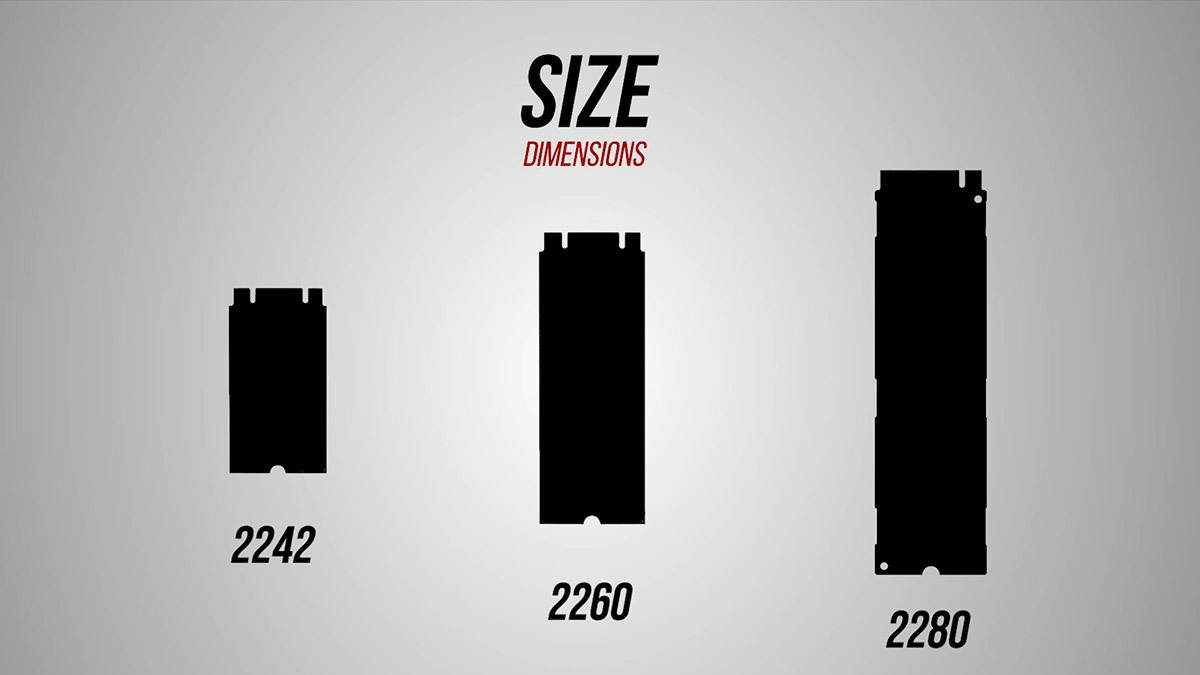
\includegraphics[scale=0.25]{images/dimensiones.jpg}
	\end{figure}
	

\end{justify}

\newpage
\noindent
\section{Como se gestiona la memoria en un computador} \label{contenido}

\begin{justify}
	
	\begin{center}
		\textbf{Gestión de Memoria de un Computador}
	\end{center}
	
	\noindent
	De forma simplificada se trata de proveer mecanismos para asignar secciones de memoria a los programas que las solicitan, y a la vez, liberar las secciones de memoria que ya no se utilizan para que estén disponibles para otros programas.\cite{septima}\\
	
	\noindent
	La memoria es uno de los principales recursos de la computadora, la cual debe de administrarse con mucho cuidado. Aunque actualmente la mayoría de los sistemas de cómputo cuentan con una alta capacidad de memoria, de igual manera las aplicaciones actuales tienen también altos requerimientos de memoria, lo que sigue generando escasez de memoria en los sistemas multitarea y/o multiusuario. \\
	
	\noindent
	La parte del sistema operativo que administra la memoria se llama administrador de memoria y su labor consiste en llevar un registro de las partes de memoria que se estén utilizando y aquellas que no, con el fin de asignar espacio en memoria a los procesos cuando éstos la necesiten y liberándola cuando terminen.\\
	
	\noindent
	\textbf{Características} \\
	
	\begin{itemize}
		\item \textbf{Protección:} La protección de memoria es un método para controlar el uso de memoria en una computadora, y es parte esencial de prácticamente todos los sistemas operativos modernos. El principal propósito de la protección de memoria es evitar que un proceso en un sistema operativo acceda a la memoria que no le ha sido asignada.
		
		\item \textbf{ Memoria compartida:} Aunque la memoria utilizada por diferentes procesos suele estar protegida, algunos procesos puede que sí tengan que compartir información y, para ello, han de acceder la misma sección de memoria. La memoria compartida es una de las técnicas más rápidas para posibilitar la comunicación entre procesos.
		
		\item \textbf{Organización lógica:} Permiten que los programas se escriban como módulos compilables y ejecutables por separado.
		
		\item \textbf{Organización física:} La memoria suele dividirse en un almacenamiento primario de alta velocidad y uno secundario de menor velocidad.  La gestión de memoria del sistema operativo se ocupa de trasladar la información entre estos dos niveles de memoria.
	\end{itemize}
		
\end{justify}

\newpage
\noindent
\section{¿Qué hace que una memoria sea más rápida que otra? ¿Por qué esto es importante?}\label{contenido}

\begin{justify}
	
	\noindent
	La \textbf{memoria RAM} tiene varios elementos que afectan al rendimiento del equipo. Por un lado, tenemos la \textbf{capacidad} de la misma: cuanto mayor sea la capacidad, mejor. Esto se debe a que podremos almacenar más datos sin tener que paginar o recurrir a otras técnicas que pueden lastrar el rendimiento. La \textbf{frecuencia} es otro de los elementos más importantes de la memoria RAM, ya que cuanto mayor sea la velocidad de la memoria, más rápido podrá trabajar los datos.\\
	
	\noindent
	Otro elemento importante en la memoria RAM al jugar, que suele ser ignorado por muchos usuarios, es el \textbf{voltaje}. Aunque no afecta directamente el rendimiento, un mayor voltaje generará mayor temperatura de las memorias. Además, conforme el voltaje aumente, menor vida útil le esperan a nuestras memorias.\\

	\begin{center}
		\textbf{La latencia es fundamental si queremos el mejor rendimiento}
	\end{center}

	\noindent
	Por último, otro elemento vital de la RAM para conseguir el mejor rendimiento posible es la latencia. En términos generales, la latencia es el tiempo que transcurre desde que la memoria recibe un comando, hasta que lo ejecuta. Dicho en otras palabras, la latencia de la RAM es el intervalo de tiempo entre las dos acciones; cuanto más bajo sea este valor, mejor. Erróneamente se ha creído que, \textbf{a medida que evolucionaba la tecnología} (DDR1, DDR2, DDR3, DDR4, etc) \textbf{aumentaba la latencia}, y eso era cada vez peor para los sistemas.\cite{octava}\\
	
	\noindent
	En realidad, la latencia real de una memoria RAM se calcula multiplicando el tiempo de ciclo del reloj, en nanosegundos, por el número de ciclos de reloj, CL, necesario para procesar el comando.\\
	
	\noindent
	De esta manera podemos ver que, por ejemplo, \textbf{una memoria RAM DDR1} a 400 MHz y una latencia CL3 \textbf{tiene más latencia real} (en nanosegundos, concretamente 15 ns) que una memoria RAM DDR4 a 2666 MHz con latencia CL18, que tiene una latencia real de 13.50 ns. Dejando las fórmulas de lado, una forma muy rápida de saber qué memoria RAM es mejor es dividir la latencia CAS entre la frecuencia en MT/s y multiplicar por 2000.\\
	Quien obtenga un valor menor significa que ofrecerá mejor rendimiento, aunque no es una ciencia exacta.\\
		 
\end{justify}

\begin{thebibliography}{0}
	
	
	\bibitem{primera}
	Maria Jose Gallegos Salgado\\
	\url{ https://es.slideshare.net/MaryJoseSg/memoria-de-una-computadora }\\
	10 de marzo de 2017
	
	\bibitem{segunda}
	María Estela Raffino\\
	\url{ https://concepto.de/memoria-cache/#ixzz6XCWM3kiX }\\
	30 de junio de 2020
	
	\bibitem{tercera}
	Uruguay OC\\
	\url{ https://uruguayoc.com/2018/03/18/que-es-el-cache-l1-l2-y-l3-en-los-procesadores/}\\
	18 marzo de 2018
	
	\bibitem{cuarta}
	Isidro Rios\\
	\url{ https://www.muycomputer.com/2018/11/04/memoria-ram-que-es-recomendaciones/r}\\
	4 de Noviembre de 2018
	
	\bibitem{quinta}
	YÚBAL FM\\
	\url{ https://www.xataka.com/basics/hdd-vs-ssd }\\
	1 de Octubre de 2018
		
	\bibitem{septima}
	Yanneth Gutiérrez Sánchez\\
	\url{https://sites.google.com/site/sisoper1/home}\\
	14 de Abril de 2013
	
	\bibitem{octava}
	Rubén Velasco\\
	\url{ https://hardzone.es/reportajes/comparativas/latencia-velocidad-ram-jugar/}\\
	11 de agosto de 2020\\
	
	
	
\end{thebibliography}



\end{document}